% Commands:
%
% * EtherstubManager._create( name );
% * VnicManager._create( name, temporary, parent );
%
% * one worker instantiation: switch + 2 appliances + communication     (sim)
% * two workers instantiation: (dou)


\documentclass{beamer}

\usepackage[polish]{babel}
\usepackage[utf8]{inputenc}
\usepackage[T1]{fontenc}
\usepackage{hyperref}
\usepackage{graphicx}
\usepackage{multicol}
\usepackage{tabularx}
\usepackage{tikz}

\usetikzlibrary{positioning}

\mode<presentation>{\usetheme{Rochester}}
\setbeamercovered{dynamic}

\title{Component-based system for management of multilevel virtualization of networking resources}
\subtitle{System komponentowy wspomagający wielopoziomową wirtualizację zasobów sieciowych}
\author{Robert Boczek \and Dawid Ciepliński}
\institute{AGH University of Science and Technology \\ ~ \\ Faculty of Electrical Engineering, Automatics, Computer Science and Electronics \\ ~ \\ Department of Computer Science \\ ~ \\ Kraków, Poland}
\date{28.09.2011}

\begin{document}

	\begin{frame}
		\titlepage
	\end{frame}


	\begin{frame}{Agenda}

		\begin{itemize}
			\item<1-> General information
			\item<2-> Motivation
			\item<3-> Thesis aim
			\item<4-> The CM4J system presentation ( Core, Gui )
			\item<5-> Tests results
			\item<6-> Summary
		\end{itemize}

	\end{frame}

	\begin{frame}{Agenda}

		\begin{itemize}
			\item \textbf{General information}
			\item Motivation
			\item Thesis aim
			\item The CM4J system presentation ( Core, Gui )
			\item Tests results
			\item Summary
		\end{itemize}

	\end{frame}

	\begin{frame}{General information}

		\begin{itemize}
			\item Project initailly started //tutaj bys napisal co robiles u jarzaba i jak zetknales sie z jimsem
			
			\item Supervisor: \textbf{prof. dr hab. inż. Krzysztof Zieliński}
			\item Technical supervisor: \textbf{mgr Marcin Jarząb}
		\end{itemize}

	\end{frame}

	\begin{frame}{Agenda}

		\begin{itemize}
			\item General information
			\item \textbf{Motivation}
			\item Thesis aim
			\item The CM4J system presentation ( Core, Gui )
			\item Tests results
			\item Summary
		\end{itemize}

	\end{frame}

	\begin{frame}{Motivation}
		\begin{itemize}
			\item Interest in distributed systems, computer networking
			\item Lack of applications offering creation of virtualized networks
			\item Desire to learn the crossbow library and Solaris OS
		\end{itemize}
	\end{frame}

	\begin{frame}{Agenda}

		\begin{itemize}
			\item General information
			\item Motivation
			\item \textbf{Thesis aim}
			\item The CM4J system presentation ( Core, Gui )
			\item Tests results
			\item Summary
		\end{itemize}

	\end{frame}

	\begin{frame}{Thesis aim}
		\begin{itemize}
			\item "There exists a component-based architecture which enables construction of a system that would facilitate working with fully isolated virtualized network resources grouped in projects"
		\end{itemize}
	\end{frame}

	\begin{frame}{Agenda}

		\begin{itemize}
			\item General information
			\item Motivation
			\item Thesis aim
			\item \textbf{The CM4J system presentation ( Core, Gui )}
			\item Tests results
			\item Summary
		\end{itemize}

	\end{frame}

	\begin{frame}{The CM4J system presentation}

		Tu generalnie o stworzonym systemie

	\end{frame}

	\begin{frame}{The CM4J system presentation - GUI}

		\begin{columns}[c]
		\column{1.5in}
			\begin{itemize}
				\item Designing desired network structure with requested virtual appliances,
				\item Discovering and modifying already created projects,
				\item Monitoring ( charts )
				\item Automatic logging using Secure Shell (SSH)
			\end{itemize}
		\column{1.5in}
			\framebox{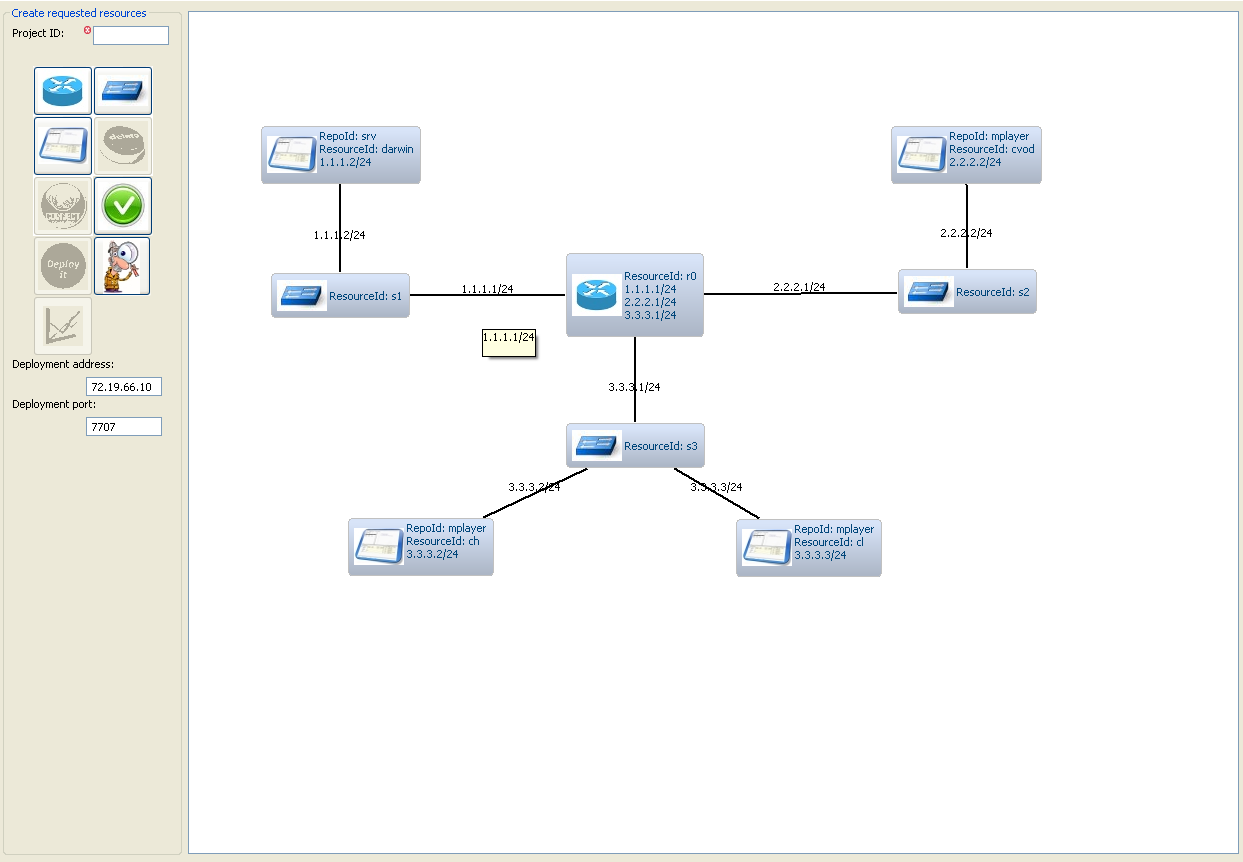
\includegraphics[width=1.5in]{img/gui-design.png}}
		\end{columns}

	\end{frame}

	\begin{frame}{Agenda}

		\begin{itemize}
			\item General information
			\item Motivation
			\item Thesis aim
			\item The CM4J system presentation ( Core, Gui )
			\item \textbf{Tests results}
			\item Summary
		\end{itemize}

	\end{frame}

	\begin{frame}{Tests results}

		System tested with respect for:
		\begin{itemize}
			\item{\only<1->{Facilitating working with virtualized network resources}}
			\item{\only<2->{Fault tolerance}}
			\item{\only<3->{Scalability ( working on many physical machines )}}
		\end{itemize}
	\end{frame}

	\begin{frame}{Tests results}

		\begin{itemize}
			\item Prepared multimedia test case
			\item Streaming server and VOD server
			\item Client differentiation
			\item Different scenarios used
		\end{itemize}

	\end{frame}

	\begin{frame}{Tests results}
		
		\begin{figure}
		   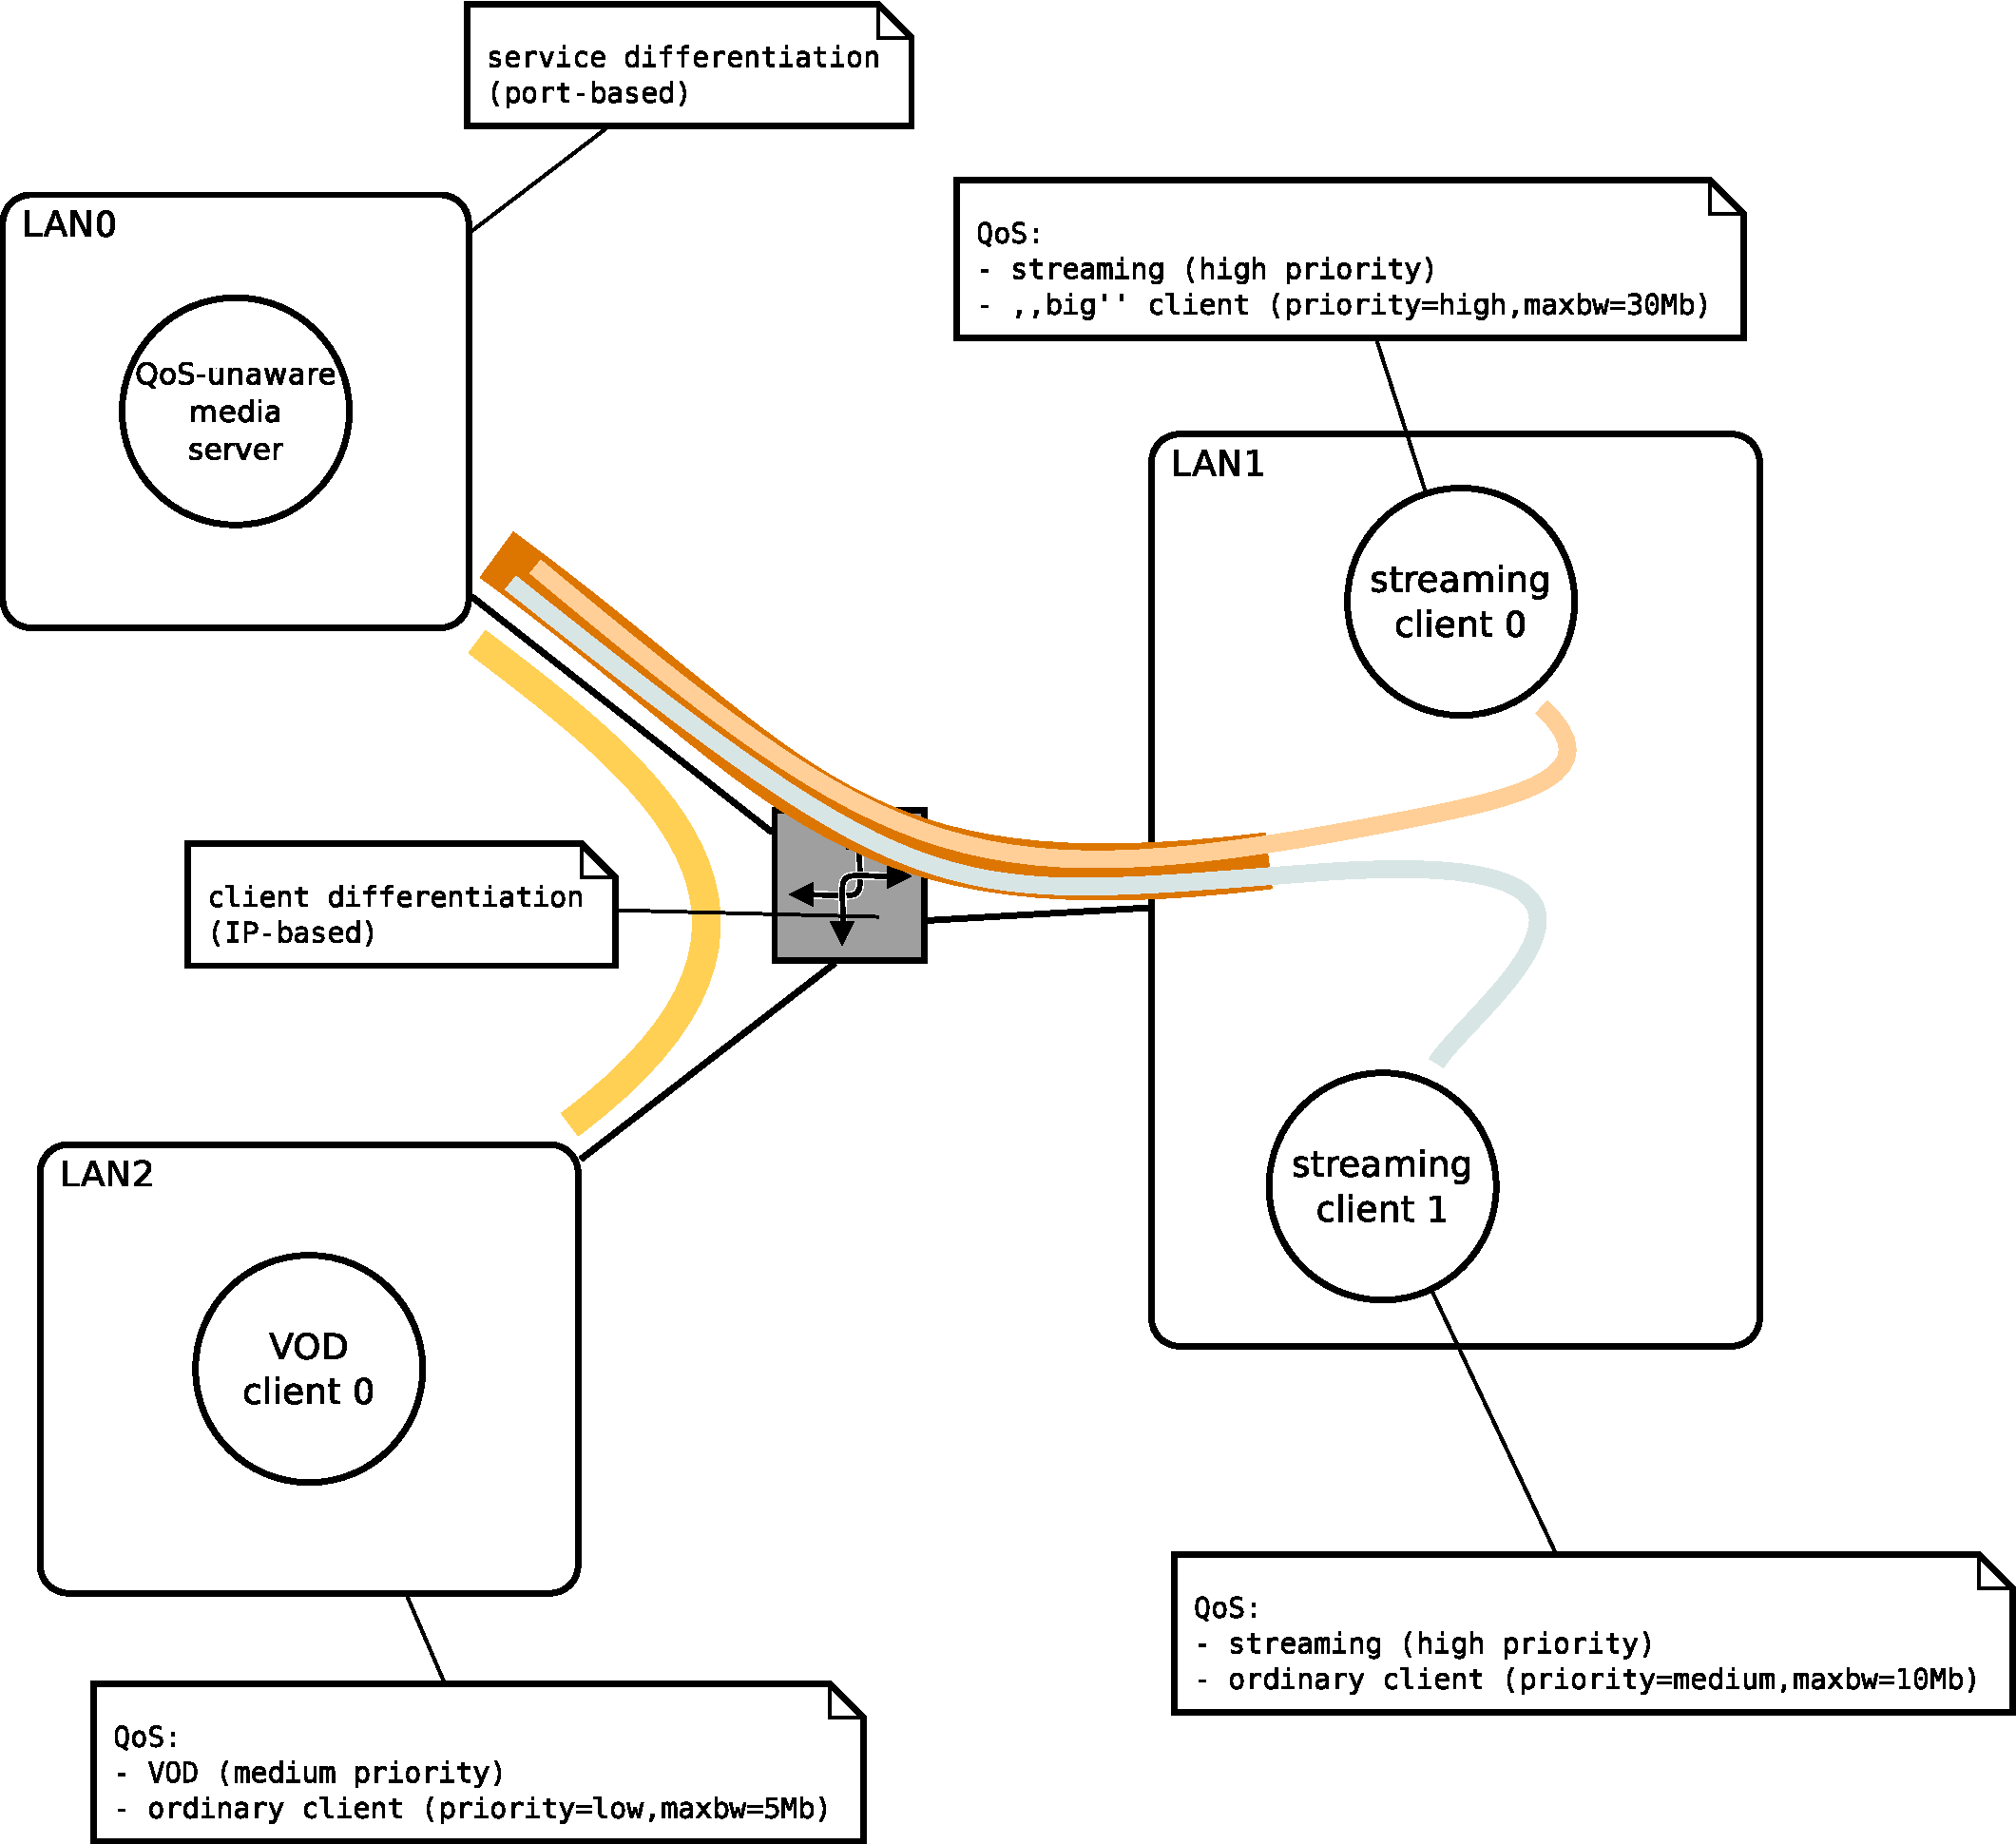
\includegraphics[width=0.65\textwidth]{img/diagram.pdf}
		\end{figure}

	\end{frame}

	\begin{frame}{Tests results}

		Tests evaluation:
		\begin{itemize}
			\item Topology design created with GUI
			\item Online modifications performed
			\item Monitoring
			\item Fault tolerance for basic errors
			\item Run on single and multiple machines
		\end{itemize}

	\end{frame}

	\begin{frame}{Agenda}

		\begin{itemize}
			\item General information
			\item Motivation
			\item Thesis aim
			\item The CM4J system presentation ( Core, Gui )
			\item Tests results
			\item \textbf{Summary}
		\end{itemize}

	\end{frame}

	\begin{frame}{Summary}

		
		\begin{itemize}
			\item Prepared complete software system 
			\item Met every production process step: requirements analysis, feasibility analysis, architecture design, implementation, test
			\item Master of science thesis creation
			\item Thesis statement proved by performed tests
			\item Expectations for future system's utilization together with JIMS
		\end{itemize}

	\end{frame}



\end{document}

